\documentclass[11pt]{article}
%\usepackage{aistats2014}

\usepackage{fullpage,color}
\usepackage{graphicx,amsmath,framed} % jeffe,handout,handout  ,
\usepackage{algorithm2e,framed}
% ge[utf8]{inputenc}		% Allow some non-ASCII Unicode in source
\usepackage{amsfonts,amssymb,hyperref}
\usepackage{framed}
\usepackage{natbib}
\usepackage{wrapfig,multirow}
\newtheorem{lemma}{Lemma}
\newtheorem{theorem}{Theorem}
\newtheorem{proof}{Proof}
\newtheorem{answer}{Answer}
\newtheorem{corollary}{Corollary}
\newtheorem{definition}{Definition}
\linespread{1.2}
\newif\iflogvar
\logvartrue

\begin{document}


\title{Crowdsourcing Algorithms: \\Summary and Comparisons}
\author{Daniel Khashabi, Stephen Mayhew}
\maketitle


\section{Introduction}
Given a specific setting for the crowdsourcing task\footnote{\texttt{http://web.engr.illinois.edu/~swoh/courses/IE598/hw/project2015.pdf}}, we implemented many methods, and attempted a few approaches which are of slight interest. 

%\textbf{Problem definition and notation: }
%Define: 
%
%$t_i \in \{ +1, -1 \} $: variables of interest to be predicted
%
%$p_j \in [0,1]$: Latent variable 
%
%$A_{ij}\in \{+1, -1\}$: Observations 
%
%$
%g_{ij}(t_i,p_j) = p_j^ {  \mathbf{I} \lbrace A_{ij} = t_i \rbrace } \times (1-p_j)^{ \mathbf{I} \lbrace A_{ij} \neq t_i \rbrace}
%$


\section{Methods}

\subsection{Majority Voting and Power Iteration}
The two simplest baselines are majority voting (stylized as \texttt{mv} in our code) and the singular value approach, which we call \texttt{power\_iteration}. This latter approach is to simply take the leading left singular eigenvector of the matrix $A$. We found that we needed to do some fiddling with the eigenvector because it would randomly be flipped all negative.


\subsection{Belief Propagation and variants}

Following from \cite{karger2014budget}, we begin with the following BP updates:
\begin{align*}
y^{(k)}_{a \to i}(p_a) &\propto \mathcal{F}(p_a) \prod_{j \in \partial a \backslash i} \left\{(p_a + \bar{p}_a + (p_a - \bar{p}_a)A_{ja})x_{j\to a}^{(k)}(+1) + (p_a + \bar{p}_a - (p_a - \bar{p}_a)A_{ja})x_{j\to a}^{(k)}(-1)  \right\}\\
x^{(k+1)}_{i \to a}(\hat{t}_i) &\propto \prod_{b \in \partial i\backslash a} \int \Big(y_{b \to i}^{(k)}(p_b)(p_b \mathbb{I}_{(A_{ib}=\hat{t}_i)} + \bar{p}_b \mathbb{I}_{(A_{ib}\neq\hat{t}_i)})\Big)dp_b
\end{align*}

With the Haldane prior, these updates collapse into a simple iterative algorithm, as seen in \cite{karger2014budget}. In our implementation, we refer to this algorithm as \texttt{simplified\_bp}. We found this was quite slow, although it may have been poor implementation. 

However, the Haldane prior is much too simple, and we would like to have a way to incorporate a better guess at the priors (especially when we know that the prior is a Beta distribution). But there is a problem with implementing the above updates directly: the continuous $p_j$'s. A simple solution is to discretize each $p_j$ into several chunks, and thereby crudely approximate the integral. We did this, and the second update became:
\begin{align*}
x^{(k+1)}_{i \to a}(\hat{t}_i) &\propto \prod_{b \in \partial i\backslash a} \sum_{p_b \in P} \Big(y_{b \to i}^{(k)}(p_b)(p_b \mathbb{I}_{(A_{ib}=\hat{t}_i)} + \bar{p}_b \mathbb{I}_{(A_{ib}\neq\hat{t}_i)})\Big)
\end{align*}

where $P=\{p_1, p_2, ..., p_k\}$. We found that this was very slow, although this may be due to a poor implementation. In our code, we refer to the implementation as \texttt{discretized\_bp}. 


\subsection{Expectation-Maximization}
We implemented the EM derivation found in the slides\footnote{\texttt{http://web.engr.illinois.edu/~swoh/courses/IE598/handout/crowd.pdf}}:

\noindent\textbf{E-Step:} 
\[q_i(t_i) = \mu_p(t_i \mid A)\]
\textbf{M-Step:} 
\[
p_j = \frac{\sum_{i \in \partial j} q_i(A_{ij})}{| \partial j |}
\]

This implementation is called \texttt{em} in our code.

Further, we derived a version of EM that included Beta priors (see the appendix for full derivation).
\[
p_j = \frac{ \alpha_j - 1 + \sum_jq(A_{ij}) }{ \alpha_j + \beta_j-2 + \sum_jq(A_{ij})  + \sum_j q(-A_{ij})  }
\]

This implementation is called \texttt{em\_with\_priors} in our code. (In implementation, we used $\alpha = 6$ and $\beta = 2$, because this is how the data was created. This seems like cheating, but we think of it as though we made an exceptionally good guess).

\subsection{HITS}

Hyperlink-Induced Topic Search (HITS), also known as hubs and authorities, is a simple web ranking algorithm that is often used in trustworthiness applications, which are very similar to crowdsourcing problems. A full derivation is given in \cite{kleinberg1999authoritative}, but by way of completeness, we give a quick overview here. 

Given a graph, the algorithm finds a hub score and an authority score for each node. Originally the nodes were webpages and the graph had no particular pattern; in this case, we have worker nodes and task nodes, and the graph is bipartite. 

We initialize $y$ in some suitable fashion, and then iterate:

\[ x^{(p)} = \sum_{q:(q,p)\in E} y^{(q)} \]
\[ y^{(p)} = \sum_{q:(p,q)\in E} x^{(q)} \]

normalizing the $x$ and $y$ vectors at each iteration. 

Although HITS is very similar to simplified BP, it is important to note that HITS operates on a different graph. Where simplified BP produces results close to the leading singular eigenvector at of the adjacency matrix, $A \in \{0, -1, 1\}^{(m\times n)}$, HITS produces results equal to the principal eigenvector of the adjacency matrix $A \in \{0, 1\}^{(m\times n)}$.

Ini our implementation of HITS, since we generate the graph in the form used by simplified BP (that is, with negative values), we need to perform a simple rewrite. With matrix dimensions given as $m \times n$, we expand it to $m \times 2n$, such that each column becomes two columns. Each $-1$ becomes $[1~~ 0]$ and each $1$ becomes $[0~~ 1]$. 

In our code, this algorithm is referred to as \texttt{hits}. 

\begin{figure}[t]
\centering
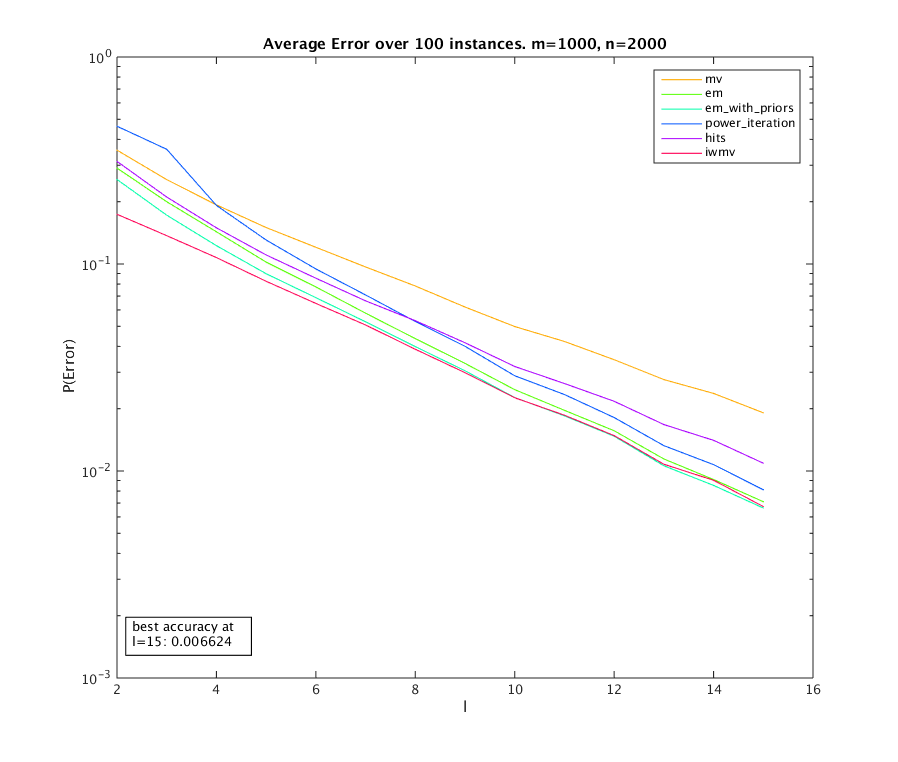
\includegraphics[scale=0.7]{all.png}
\caption{Many runs at high parameter values.}
\label{fig:all}
\end{figure}

\subsection{Iterative Weighted Majority Voting}

We also implemented the algorithm found in \cite{li2014error}, which is basically hard EM, with an added step which rescales the estimated worker weights $w_i$:

\[ \nu_i = Lw_i - 1 \]

In this case, $L=2$, which is reminiscent of the $q$ variable measuring quality in \cite{karger2014budget}. The reasoning given is also similar. Estimated weights close to 0.5 (that is, close to random) will be pushed to 0, and higher weights will be rewarded. $\nu_i$ are then used as the weights for weighted majority voting.

We refer to this algorithm as \texttt{iwmv} in our code.

\begin{figure}[t]
\centering

\includegraphics[scale=0.3]{missing.png}
\caption{Simplified BP with manageable parameters. (Missing... as of writing, this graphic is not available because of computer issues)}
\label{fig:simp}
\end{figure}

\section{Experiments}
We implemented these algorithms in matlab. We ran \texttt{mv}, \texttt{em}, \texttt{em\_with\_priors}, \texttt{power\_iteration}, \texttt{hits}, \texttt{iwmv} together with the full parameters specified in the problem statement. That is, $n=2000$ averaged over $100$ instances. See Figure \ref{fig:all} for a plot of these algorithms.

\texttt{simplified\_bp} and \texttt{discretized\_bp} were too slow to run on the full parameter set, so we ran them on smaller parameter sizes to get an estimate for the scores. See Figure \ref{fig:simp} for \texttt{simplified\_bp} and Figure \ref{fig:disc} for \texttt{discretized\_bp}.

For the discretized BP case, as seen in Figure \ref{fig:disc}, we discretized the interval $[0,1]$ with 10 chunks and some slight rounding to avoid 0 and 1 (which have 0 probabilities in the Beta distribution). The final error probability is 0.006346, which is slightly better than the best result of all the other algorithms on the much larger problem size. 

We were surprised that \texttt{iwmv} should work so well. 

All of our code is available on GitHub\footnote{\texttt{https://github.com/mayhewsw/crowdsourcing/}}.

\section{Further Work}
We put considerable time into implementations of tree-reweighted message passing (see \cite{kolmogorov2006convergent}), and spectral initialization for EM (see \cite{zhang2014spectral}). However, neither of them came to fruition as of the time of writing (perhaps we can work out the bugs before the presentation in 12 hours). We were attempting to use opengm\footnote{\texttt{http://hci.iwr.uni-heidelberg.de/opengm2/}}.




\begin{figure}[t]
\centering
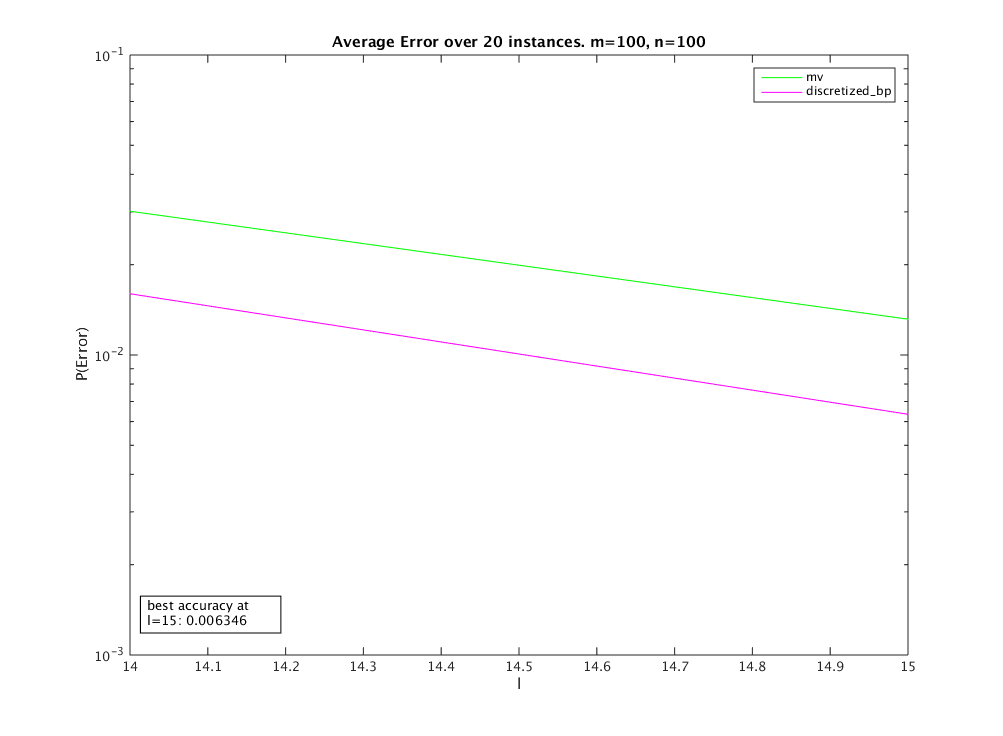
\includegraphics[scale=0.5]{mv_discretized.png}
\caption{Majority Voting and Discretized BP. (This is over a small problem size, and only for $\ell=14$ and $\ell=15$ because of slow running times)}
\label{fig:disc}
\end{figure}

%\section*{Acknowledgment}
%The authors would like to thank Ke Jiang for providing the the data used in their work. We also thank Shyam Upadhyay and Daphne Tsatsoulis for helpful comments on the draft. 

\bibliographystyle{apalike}
% argument is your BibTeX string definitions and bibliography database(s)
\bibliography{ref}

\clearpage
\section{Appendix}

%\subsection{BP Stuff}
%$$
%\psi_{ij}(t_i, p_j) = p_j \mathbf{I} \left\lbrace  A_{ij}=  t_i  \right\rbrace +  (1-p_j ) \mathbf{I} \left\lbrace  A_{ij} \neq  t_i  \right\rbrace
%$$
%
%$$
%\mathbb{F}_{mf}(b) = \sum_{(i, j) \in E} \sum_{t_i, p_j} b_i^L(t_i) b_j^R(p_j) \psi_{ij}(t_i, p_j) + \sum_{i \in V_L} \sum_{t_i} b_i^L(t_i)  \ln b_i^L(t_i) +  \sum_{j \in V_R} \sum_{p_j} b_j^R(p_j)  \ln b_j^R(p_j)
%$$
%$$
%\mathcal{L} = \mathbb{F}_{mf}(b) - \sum_{i \in V_L} \lambda_i^L \left\lbrace  \sum_{t_i} b_i^L(t_i)  - 1  \right\rbrace - \sum_{j \in V_R} \lambda_j^R \left\lbrace  \sum_{p_j} b_j^R(p_j)  - 1  \right\rbrace
%$$
%
%$$
%\begin{cases}
%\frac{\partial \mathcal{L}}{\partial b_i^L} = \sum_{j \in V_R} \sum_{p_j}  b_j^R(p_j) \psi_{ij}(t_i, p_j) +  b_i^L(t_i) +1 - \lambda_i^L  = 0 \\ 
%\frac{\partial \mathcal{L}}{\partial b_j^R} = \sum_{i \in V_L} \sum_{t_i}  b_i^L(t_i) \psi_{ij}(t_i, p_j) +  b_j^R(p_j) +1 - \lambda_j^R  = 0  
%\end{cases}
%$$
%
%$$
%\Rightarrow  
%\begin{cases}
%b_i^L(t_i) \propto  \exp \left\lbrace  - \sum_{j \in V_R} \sum_{p_j}  b_j^R(p_j) \psi_{ij}(t_i, p_j) \right\rbrace \\ 
%b_j^R(p_j) \propto \exp \left\lbrace  - \sum_{i \in V_L} \sum_{t_i}  b_i^L(t_i) \psi_{ij}(t_i, p_j)   \right\rbrace 
%\end{cases}
%$$
%

\subsection*{EM derivation}
Consider having the following prior on each $p_j$: 
$$
c + (1-c)Z_j, \quad \text{ where } Z_j \sim \text{Beta}(\alpha_j, \beta_j) 
$$
The full likelihood: 
$L(p; t) = \prod_{i,j} g_{ij}(t_i,p_j) \prod_j \left( c+ \frac{1-c}{B(\alpha_j, \beta_j)} p_j^{\alpha_j-1} (1-p_j)^{\beta_j-1}  \right) $

The likelihood for worker $j$: 
\begin{align*}
L_j(p; t) &= \prod_{i} g_{ij}(t_i,p_j) \left( c+ \frac{1-c}{B(\alpha_j, \beta_j)} p_j^{\alpha_j-1} (1-p_j)^{\beta_j-1}  \right) \\
&= \frac{1-c}{B(\alpha_j, \beta_j)}p_j^{ \alpha_j-1 + \sum_i \mathbf{I} \lbrace A_{ij} = t_i \rbrace }  (1-p_j)^{ \beta_j-1 + \sum_i \mathbf{I} \lbrace A_{ij} \neq t_i \rbrace } + cp_j^{\sum_i \mathbf{I} \lbrace A_{ij} = t_i \rbrace } (1-p_j)^{  \sum_i \mathbf{I} \lbrace A_{ij} \neq t_i \rbrace } 
\end{align*}

\textbf{E-step:} 

Suppose $t_i \sim q_i$. Then:
\begin{align*}
Q_j(p) =\mathbb{E}_{t}\left[ \ln L_j(p; t) \right] = \sum_tq(t) \Bigg[&  
\ln \frac{1-c}{B(\alpha_j, \beta_j)} + \left(  { \alpha_j-1 + \sum_i \mathbf{I} \lbrace A_{ij} = t_i \rbrace } \right)  \ln p_j  \\ &+ \left( { \beta_j-1 + \sum_i \mathbf{I} \lbrace A_{ij} \neq t_i \rbrace } \right) \ln (1-p_j)  \\ 
&+ \ln c + \left( \sum_i \mathbf{I} \lbrace A_{ij} = t_i \rbrace \right) \ln p_j + \left( {  \sum_i \mathbf{I} \lbrace A_{ij} \neq t_i \rbrace } \right) \ln (1-p_j) \Bigg], 
\end{align*}
which can be simplified to
\begin{align*}
Q_j(p) =   
\ln \frac{1-c}{B(\alpha_j, \beta_j)}  + \ln c +  \left(   \alpha_j-1 \right)  \ln p_j  + \left( \beta_j - 1  \right) \ln (1-p_j) +  \Bigg[&  
\ln p_j \sum_i q(A_{ij}) +  \ln (1-p_j) \sum_i q(-A_{ij}) \Bigg], 
\end{align*}

where 
$$
q_i(t_i) = \frac{ \prod_{j} g_{ij}(t_i, p_j) }{ \sum_{t_i} \prod_{j} g_{ij}(t_i, p_j)   }  \quad \quad (1)
$$

\textbf{M-step: }
Taking derivative with respect to $p_j$: 
$$
\frac{\partial Q_j}{\partial p_j} = \frac{\alpha_j - 1 + \sum_jq(A_{ij})}{p_j} + \frac{\beta_j-1  + \sum_j q(-A_{ij}) }{1-p_j} = 0
$$
which results in 
$$
p_j = \frac{ \alpha_j - 1 + \sum_jq(A_{ij}) }{ \alpha_j + \beta_j-2 + \sum_jq(A_{ij})  + \sum_j q(-A_{ij})  }
$$

\end{document}
